\documentclass[11pt,a4paper]{article}
\usepackage[T1]{fontenc}
\usepackage{lmodern}
\usepackage[margin=1.7cm,top=2.2cm,bottom=2cm]{geometry}
\usepackage{graphicx}
\usepackage[table]{xcolor}
\usepackage{tikz}
\usepackage{fancyhdr}
\usepackage[most]{tcolorbox}
\usepackage{microtype}
\definecolor{navy}{RGB}{21,45,99}
\definecolor{ocean}{RGB}{28,97,158}
\definecolor{aqua}{RGB}{0,142,150}
\definecolor{sky}{RGB}{235,243,252}
\definecolor{ink}{RGB}{40,40,50}
\renewcommand{\familydefault}{\sfdefault}
\color{ink}
\pagestyle{fancy}\fancyhf{}
\renewcommand{\headrulewidth}{0pt}
\fancyhead[L]{\small\color{navy}\textbf{Module 4: Malicious Software} \,\textbar\, Lecture Notes}
\fancyhead[R]{
\includegraphics[height=0.75cm]{../au_logo.png}}
\fancyfoot[C]{\small\color{ocean}\thepage}
\setlength{\parindent}{0pt}
\newtcolorbox{slidebox}[3]{enhanced,breakable=false,colback=white,colframe=ocean,boxrule=0.6pt,arc=2mm,
  left=3mm,right=3mm,top=2mm,bottom=2mm,
  title={\textbf{Slide #1}\;\,|\;\,#2\quad\normalfont\small(about #3 seconds)},
  fonttitle=\sffamily\color{white},colbacktitle=navy,attach boxed title to top left={yshift=-2mm,xshift=3mm},
  boxed title style={arc=1.5mm,colback=navy},before skip=5mm,after skip=3mm}
\begin{document}
\thispagestyle{empty}
\begin{tikzpicture}[remember picture,overlay]
  \fill[navy] (current page.north west) rectangle ([yshift=-9.5cm]current page.north east);
  \fill[aqua] ([yshift=-9.5cm]current page.north west) rectangle ([yshift=-9.7cm]current page.north east);
  \node[anchor=north east] at ([xshift=-1.5cm,yshift=-1.2cm]current page.north east) {
\includegraphics[height=2.4cm]{../au_logo.png}};
  \node[anchor=west,white,font=\large] at ([xshift=1.8cm,yshift=-2.2cm]current page.north west) {NETWORK SECURITY \,\textbar\, MODULE 4};
  \node[anchor=west,white,font=\fontsize{30}{36}\selectfont\bfseries] at ([xshift=1.8cm,yshift=-4.2cm]current page.north west) {Lecture Notes};
  \node[anchor=west,white,font=\Large] at ([xshift=1.8cm,yshift=-5.6cm]current page.north west) {Malicious Software};
  \node[anchor=west,white,font=\normalsize,align=left] at ([xshift=1.8cm,yshift=-7.2cm]current page.north west)
    {Lesson 6: Viruses, Worms and Trojan Horses};
\end{tikzpicture}
\vspace*{8.6cm}

\begin{tcolorbox}[colback=sky,colframe=ocean,arc=2mm,title=\textbf{How to use these notes},fonttitle=\sffamily]
\begin{itemize}\setlength{\itemsep}{3pt}
  \item There is \textbf{one note for each of the 48 slides}, in the same order as \texttt{module4.pdf}. A small picture of the slide sits beside each note.
  \item The notes are written \textbf{from teacher to students} in \textbf{simple language}: read them aloud as they are, or use them as a guide in your own words.
  \item Each note takes \textbf{at most 2 minutes} to speak (about 140--170 words, roughly 1--1\textonequarter{} minutes) at a steady classroom pace of about 135 words per minute. The estimate for each slide is shown in its title bar.
  \item Phrases such as ``look at the diagram'' tell you when to point at the slide.
\end{itemize}
\end{tcolorbox}

\vspace{4mm}
\begin{center}
\renewcommand{\arraystretch}{1.5}
\begin{tabular}{>{\columncolor{navy}\color{white}\bfseries}l >{\columncolor{sky}}l}
Slides & 48 \\
Total words & 7,535 \\
Estimated talking time & about 56 minutes (without pauses or questions) \\
Lesson 6 & slides 3--48 \\
\end{tabular}
\end{center}
\newpage
\begin{slidebox}{1}{Title: Malicious Software}{72}
\begin{minipage}[t]{0.40\linewidth}\vspace{0pt}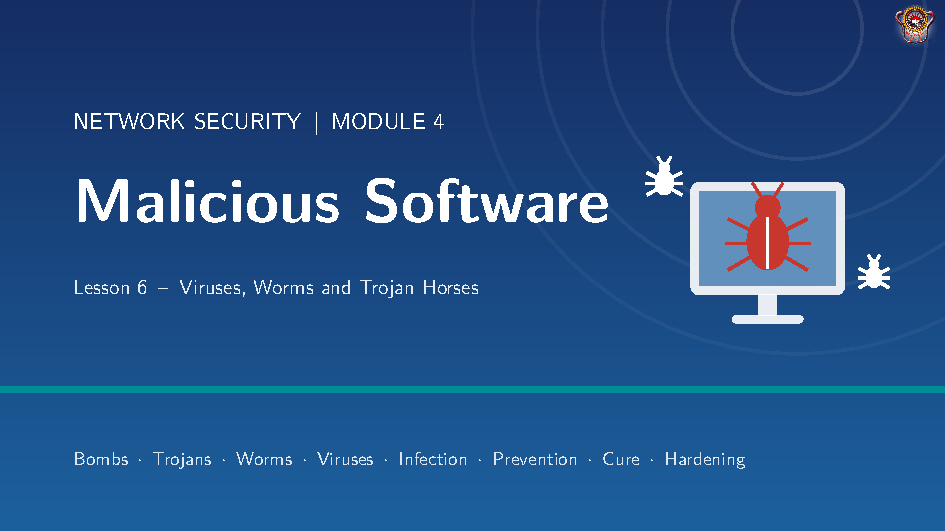
\includegraphics[width=\linewidth,page=1]{../module4.pdf}\end{minipage}\hfill
\begin{minipage}[t]{0.57\linewidth}\vspace{0pt}\small\linespread{1.1}\selectfont Good morning, everyone. Today we begin Module 4, Malicious Software. Malicious means harmful or with bad intention. So malicious software is software that is written to do harm. Look at the picture on the right. There is a computer screen with a big red bug in the middle, and small bugs crawling around it. In computer language, we often call these harmful programs bugs, viruses or worms. This whole module comes from one lesson in your study material, Lesson 6, Viruses, Worms and Trojan Horses. At the bottom of the slide you can see the topics we will cover: bombs, Trojans, worms, viruses, how infection happens, how to prevent it, how to cure it, and how to harden, or strengthen, our systems. I am sure many of you have already faced a virus on your phone or laptop. So this module is very practical. By the end of today, you will know how these programs work and how to protect yourself from them.\end{minipage}
\end{slidebox}
\begin{slidebox}{2}{Roadmap of This Module}{69}
\begin{minipage}[t]{0.40\linewidth}\vspace{0pt}\includegraphics[width=\linewidth,page=2]{../module4.pdf}\end{minipage}\hfill
\begin{minipage}[t]{0.57\linewidth}\vspace{0pt}\small\linespread{1.1}\selectfont Let me show you our road map for today. On the left side we have the first four topics. First, perverse software: what it is and why people write it. Second, the four kinds of perverse software: bombs, Trojans, worms and viruses, and how they are different. Third, the evolution and menace of viruses, which is the history and the danger, from 1949 up to the famous Brain virus. Fourth, the process of infection, which means how a virus actually enters and spreads inside a computer. On the right side we have four more topics. Fifth, the classification of viruses into boot, system and program infectors. Sixth, some famous viruses and the phases of a virus's life. Seventh, prevention and cure. And eighth, hardening the system and the six types of malicious code. The first half explains the enemy. The second half explains how to fight it. Keep this map in mind as we go.\end{minipage}
\end{slidebox}
\begin{slidebox}{3}{Lesson 6: Viruses, Worms and Trojan Horses}{63}
\begin{minipage}[t]{0.40\linewidth}\vspace{0pt}\includegraphics[width=\linewidth,page=3]{../module4.pdf}\end{minipage}\hfill
\begin{minipage}[t]{0.57\linewidth}\vspace{0pt}\small\linespread{1.1}\selectfont We now start Lesson 6, Viruses, Worms and Trojan Horses. Before we begin, let me ask you a question. Have you ever opened a file, and suddenly your computer became slow, or strange messages appeared, or your files disappeared? If yes, you have probably met a virus. The names in this lesson are borrowed from real life. A virus in biology is a tiny thing that enters your body and makes copies of itself. A worm moves from place to place on its own. And the Trojan horse comes from an old Greek story, which I will tell you shortly. These names are not random. Each one describes how that program behaves. If you remember the real-life meaning of each name, you will never confuse them in your examination. So let us begin our journey into the world of harmful programs.\end{minipage}
\end{slidebox}
\begin{slidebox}{4}{What You Will Learn}{69}
\begin{minipage}[t]{0.40\linewidth}\vspace{0pt}\includegraphics[width=\linewidth,page=4]{../module4.pdf}\end{minipage}\hfill
\begin{minipage}[t]{0.57\linewidth}\vspace{0pt}\small\linespread{1.1}\selectfont Let us look at what you will be able to do at the end of this lesson. Look at the five numbered points on the left. One: define computer viruses and understand how they evolved over time. Two: explain the damage a virus can do. Three: understand the process of virus infection, which means how it enters and spreads. Four: identify different types of viruses based on where they infect the computer. Five: describe and apply preventive measures, which means steps to keep viruses away. Now read the red box on the right. Your study material says the world of information technology is going through an era of electronic terrorism in the form of viruses. That is a strong statement. It means viruses are dangerous enough to stop computer systems from working properly. The blue box below shows our plan for today: evolution, menace, infection, classification, types, prevention and finally cure. We will follow this order.\end{minipage}
\end{slidebox}
\begin{slidebox}{5}{What Is Perverse Software?}{68}
\begin{minipage}[t]{0.40\linewidth}\vspace{0pt}\includegraphics[width=\linewidth,page=5]{../module4.pdf}\end{minipage}\hfill
\begin{minipage}[t]{0.57\linewidth}\vspace{0pt}\small\linespread{1.1}\selectfont The study material uses a special term: perverse software. Read the definition in the blue box. Perverse software is software which causes a perverse activity. Perverse simply means wrong, harmful or unwanted. Now, what is a perverse activity for a computer? Look at the diagram on the left. A computer has a CPU and memory in the middle, connected to input and output devices, storage, programs and data. Perverse software, shown as the red bug, sits among them and disturbs their normal work. The list on the right gives examples. It can modify or completely destroy data without the user wanting it. It can cause unpredictable behaviour, like strange things on the screen or wrong printing. And it can sabotage, or damage, the operating system itself. Finally, read the last line. A computer on which perverse software is running is called an infected system, just like a person with a virus is called infected.\end{minipage}
\end{slidebox}
\begin{slidebox}{6}{Why Is Perverse Software Written?}{68}
\begin{minipage}[t]{0.40\linewidth}\vspace{0pt}\includegraphics[width=\linewidth,page=6]{../module4.pdf}\end{minipage}\hfill
\begin{minipage}[t]{0.57\linewidth}\vspace{0pt}\small\linespread{1.1}\selectfont Why would anyone write harmful software? Look at the red circle called motives, which means reasons. Around it are five reasons from your study material. Some people do it for publicity, because they want to become famous. Some do it as a practical joke, just to have fun at others' expense. Some do it out of personal revenge against a company or a person, for example an employee who was fired. Some simply have a natural desire to tease other people. And some are just the act of a maniac, a person who enjoys causing trouble for no clear reason. Now read the red box at the bottom. Whatever the reason, the result is the same. All of them aim to produce disastrous effects. Meanwhile, the normal user only wants to do something useful and increase their productivity. So the virus writer's fun becomes the ordinary user's loss of time, data and money.\end{minipage}
\end{slidebox}
\begin{slidebox}{7}{Why Is It So Hard to Notice?}{67}
\begin{minipage}[t]{0.40\linewidth}\vspace{0pt}\includegraphics[width=\linewidth,page=7]{../module4.pdf}\end{minipage}\hfill
\begin{minipage}[t]{0.57\linewidth}\vspace{0pt}\small\linespread{1.1}\selectfont Here is an important question. If viruses are so harmful, why don't we notice them immediately? Look at the diagram. Four computers are in a row. PC A is infected, shown by the red bug. The infection quietly spreads from A to B, B to C, and C to D. But look at the green box below. Meanwhile, every PC keeps working as if nothing happened. Now read the reasons on the right. Different perverse programs do different things, but they all create uncertainty for users. The normal MS-DOS operating system was designed for bona fide users, which means honest users. It was not built to detect such harmful software. Standard security checks also do not notice the problem. So an infected system continues to work normally, and this is exactly how the infection spreads further. A virus that makes noise gets caught. A virus that stays quiet survives and spreads.\end{minipage}
\end{slidebox}
\begin{slidebox}{8}{Four Kinds of Perverse Software}{64}
\begin{minipage}[t]{0.40\linewidth}\vspace{0pt}\includegraphics[width=\linewidth,page=8]{../module4.pdf}\end{minipage}\hfill
\begin{minipage}[t]{0.57\linewidth}\vspace{0pt}\small\linespread{1.1}\selectfont Your study material divides perverse software into four kinds. Look at the tree. First, bombs, in orange. A bomb is bad code that waits for a particular time or event, and then explodes. Second, Trojan horses, in purple. A Trojan is illegal code hidden inside a program that looks legitimate. Third, worms, in teal. A worm is a stand-alone program that copies itself to other machines on the network. Fourth, viruses, in red. A virus is code that infects other programs and makes copies of itself. Now read the blue note at the bottom. In everyday conversation, people use the word virus for everything, including worms and Trojans. But in this lesson, and in your examination, we must keep them separate, because they behave differently. Over the next few slides, we will study each of the four kinds one by one, starting with bombs.\end{minipage}
\end{slidebox}
\begin{slidebox}{9}{(a) Bombs}{70}
\begin{minipage}[t]{0.40\linewidth}\vspace{0pt}\includegraphics[width=\linewidth,page=9]{../module4.pdf}\end{minipage}\hfill
\begin{minipage}[t]{0.57\linewidth}\vspace{0pt}\small\linespread{1.1}\selectfont Let us start with bombs. Read the definition in the blue box. A bomb is a piece of bad code deliberately planted by an insider or by a supplier of a program. Insider means someone inside the organization, like an employee. Look at the picture on the left. Inside the bomb, it says: if event, then damage. That is exactly how a bomb works. Now look at the points on the right. A bomb is triggered by an event, which may be logical or based on time. When the condition is met, it explodes and causes damage immediately. Now here is a very important point. A bomb cannot infect other programs. It does not spread. Look at the red text under the picture. Because it does not propagate, the chance of a large epidemic is small. It stays where it was planted. There are two types of bombs: time bombs and logic bombs, which we see next.\end{minipage}
\end{slidebox}
\begin{slidebox}{10}{Time Bomb vs. Logic Bomb}{73}
\begin{minipage}[t]{0.40\linewidth}\vspace{0pt}\includegraphics[width=\linewidth,page=10]{../module4.pdf}\end{minipage}\hfill
\begin{minipage}[t]{0.57\linewidth}\vspace{0pt}\small\linespread{1.1}\selectfont There are two types of bombs. On the left is the time bomb. Look at the clock with a red label showing a date and time. The name comes from a real time bomb, which explodes at a set time. In the same way, a computer time bomb is started by the computer clock. On a particular date and time, it does its harmful work, such as disrupting the system or changing or destroying stored data. On the right is the logic bomb. Look at the purple box. It says: if MYFILE is deleted, then overwrite memory with zeros. This is the example from your study material. A logic bomb is activated by a certain combination of events, not by time. In this example, the moment someone deletes a file named MYFILE, the whole memory is wiped out. Now read the blue box. Both types can be set to go off in the future, and both are usually planted by someone with inside access.\end{minipage}
\end{slidebox}
\begin{slidebox}{11}{(b) Trojan Horse}{70}
\begin{minipage}[t]{0.40\linewidth}\vspace{0pt}\includegraphics[width=\linewidth,page=11]{../module4.pdf}\end{minipage}\hfill
\begin{minipage}[t]{0.57\linewidth}\vspace{0pt}\small\linespread{1.1}\selectfont Now let me tell you a short story. Long ago, the Greeks were fighting the city of Troy. They could not break in. So they built a huge wooden horse and left it outside the city as a gift. The people of Troy happily pulled it inside. At night, Greek soldiers hidden inside the horse came out and captured the city. Look at the picture: the horse looks like a gift, but hides attackers inside. A Trojan horse program works exactly like this. Read the definition. It is illegal code hidden inside a legitimate program, which causes a harmful action. Now look at the points. It may change or steal passwords, or modify protected records. It hides inside a host program and usually does not damage the host. It cannot copy itself to other software. It runs only when the program is called explicitly. And it spreads only when an unsuspecting user copies the program to another system.\end{minipage}
\end{slidebox}
\begin{slidebox}{12}{Example: The Christmas Card Trojan}{70}
\begin{minipage}[t]{0.40\linewidth}\vspace{0pt}\includegraphics[width=\linewidth,page=12]{../module4.pdf}\end{minipage}\hfill
\begin{minipage}[t]{0.57\linewidth}\vspace{0pt}\small\linespread{1.1}\selectfont Here is a famous real example from your study material: the Christmas card Trojan. It was found on IBM's internal email system. Look at the diagram. A user receives the program and types the word Christmas. The program does exactly what it promised: it draws a nice Christmas tree on the screen, as you see in the middle. The user is happy. But secretly, as the red dashed arrows show, the program also sends copies of itself to every user connected to the network. Each of those users runs it, and it sends even more copies. Now read the red box. The network got flooded with so many copies that other users could not even save their half-finished work. This is a great lesson for all of you. Something that looks harmless and fun can hide a harmful action. Never run a program or open an attachment just because it looks friendly or comes with a nice message.\end{minipage}
\end{slidebox}
\begin{slidebox}{13}{(c) Worms}{69}
\begin{minipage}[t]{0.40\linewidth}\vspace{0pt}\includegraphics[width=\linewidth,page=13]{../module4.pdf}\end{minipage}\hfill
\begin{minipage}[t]{0.57\linewidth}\vspace{0pt}\small\linespread{1.1}\selectfont Now let us study worms. Look at the diagram. There are four computers connected in a network. On top of each computer is a small teal bar, which is the worm. The worm copies itself from one machine to the next, all by itself. Now read the points on the right. A worm can relocate itself, which means move from place to place, and it does not need a host program. This is a key difference. It copies itself to another machine on the network. Because worms are stand-alone programs, they are actually easier to detect than Trojans and viruses, which hide inside other programs. Worms store themselves in critical areas of the disk, and have been known to damage entire LANs, which are local area networks. Now read the blue box carefully. A Trojan needs a host and cannot replicate. A worm needs no host and can replicate. Remember this difference for your examination.\end{minipage}
\end{slidebox}
\begin{slidebox}{14}{Worms Can Also Be Useful}{71}
\begin{minipage}[t]{0.40\linewidth}\vspace{0pt}\includegraphics[width=\linewidth,page=14]{../module4.pdf}\end{minipage}\hfill
\begin{minipage}[t]{0.57\linewidth}\vspace{0pt}\small\linespread{1.1}\selectfont Here is something surprising. Worms are not always bad. Read the blue box on the left. Worms can sabotage systems, but they can also be used for useful tasks, for example while installing a network. How? You insert a worm into the network and check for its presence at each node, which means each computer. Look at the four circles. Three have green ticks, meaning the worm reached them. One has a red cross, meaning the worm never appeared there. So we can assume that node is not connected to the network properly. It is a clever way to test a network. On the right are two named examples. The Alarm Clock worm places wake-up calls on a list of users, travelling through the network to an outgoing terminal. The Existential worm has only one purpose: to stay alive. It copies itself to several places but causes no damage. So the same idea can be used for good or bad.\end{minipage}
\end{slidebox}
\begin{slidebox}{15}{(d) Viruses}{67}
\begin{minipage}[t]{0.40\linewidth}\vspace{0pt}\includegraphics[width=\linewidth,page=15]{../module4.pdf}\end{minipage}\hfill
\begin{minipage}[t]{0.57\linewidth}\vspace{0pt}\small\linespread{1.1}\selectfont Now we come to the most famous one, the virus. Look at the simple formula on the left. Trojan horse plus auto-relocation, like worms, equals virus. This comes from a definition by Davis and Gantenbein in 1987, shown in the blue box. They said a virus is a Trojan horse program with the capability of auto-relocation, and it can attack other programs. In simple words, a virus hides like a Trojan and spreads like a worm. So it combines the worst of both. Now read the points. The virus came after worms in history. It is the most dangerous perverse software, because it can reproduce itself. It attaches itself to a regularly used program, so the host looks normal and harmless. It is highly contagious, which means it spreads very easily. And it can take control of the operating system and destroy all the data and programs on your hard disk.\end{minipage}
\end{slidebox}
\begin{slidebox}{16}{A Virus Behaves Like a Parasite}{70}
\begin{minipage}[t]{0.40\linewidth}\vspace{0pt}\includegraphics[width=\linewidth,page=16]{../module4.pdf}\end{minipage}\hfill
\begin{minipage}[t]{0.57\linewidth}\vspace{0pt}\small\linespread{1.1}\selectfont A parasite is a living thing that lives on another living thing and takes food from it. A virus behaves just like a parasite. Follow the four circles from left to right. First, it draws resources. It uses the computer's own resources to watch the computer's activities. Second, it stays quiet. It does not immediately change how the system boots or works. Third, this quietness helps it evade detection, which means avoid being caught early. Fourth, it spreads first, and destroys only later. Now read the red box carefully, because this is a very clever point. Why does a virus wait? If it destroyed its host program immediately, it would also destroy itself, and it could never reproduce and spread. So a destructive virus must delay its attack. It first makes many copies on many computers, and only then does the damage. This is exactly why viruses are so dangerous: by the time you notice, they are everywhere.\end{minipage}
\end{slidebox}
\begin{slidebox}{17}{Comparing the Four Kinds (Fig. 6.1)}{68}
\begin{minipage}[t]{0.40\linewidth}\vspace{0pt}\includegraphics[width=\linewidth,page=17]{../module4.pdf}\end{minipage}\hfill
\begin{minipage}[t]{0.57\linewidth}\vspace{0pt}\small\linespread{1.1}\selectfont This table is Figure 6.1 in your study material, and it is very important for your examination. It compares the four kinds of perverse software using just two questions. First, does it require a host program? Second, can it replicate and relocate, which means copy itself and move? Let us read it row by row. A bomb: host may or may not be needed, and it cannot replicate. A Trojan: needs a host, and cannot replicate. A worm: needs no host, and can replicate. A virus: needs a host, and can replicate. Now read the memory trick in the box. A worm travels alone. A virus needs a host and spreads. Bombs and Trojans stay where they are planted. If you remember this one sentence, you can rebuild the whole table in your exam. I suggest you draw this table in your notebook right now and practise it two or three times.\end{minipage}
\end{slidebox}
\begin{slidebox}{18}{The Evolution of the Virus}{70}
\begin{minipage}[t]{0.40\linewidth}\vspace{0pt}\includegraphics[width=\linewidth,page=18]{../module4.pdf}\end{minipage}\hfill
\begin{minipage}[t]{0.57\linewidth}\vspace{0pt}\small\linespread{1.1}\selectfont Let us now look at the history of viruses. Follow the timeline from left to right. In 1949, the famous scientist John von Neumann wrote a paper about a self-replicating program, a program that can copy itself. At that time, people thought it was impossible, and the idea was dropped. Next comes Code-Wars, a game at AT and T Bell Labs. In this game, two players wrote programs that tried to destroy each other's programs. Read the blue box. The authors realized how dangerous this could be, so they kept it secret. Around the same time, students at MIT were also experimenting with programs that messed up other programs, just as a harmless hobby. These games and hobbies gave rise to the idea of computer viruses. Finally, in 1985, came the first commercial use, the Brain virus, which we see on the next slide. So an idea that started as theory and fun slowly became a real threat.\end{minipage}
\end{slidebox}
\begin{slidebox}{19}{1985: The Brain (Pakistani) Virus}{68}
\begin{minipage}[t]{0.40\linewidth}\vspace{0pt}\includegraphics[width=\linewidth,page=19]{../module4.pdf}\end{minipage}\hfill
\begin{minipage}[t]{0.57\linewidth}\vspace{0pt}\small\linespread{1.1}\selectfont In 1985, two brothers in Lahore, Pakistan, ran a shop selling low-cost software. They were worried that people were making illegal copies of their software, which we call piracy. Look at the diagram. To track piracy, they hid a small piece of code on nearly every disk they sold. This code was self-replicating, which means it could copy itself. When someone used an unauthorized copy, the code infected that person's computer and disturbed its operations. This was called the Brain virus, or the Pakistani virus. When it struck, a message appeared on the screen saying: Welcome to the Dungeon. Now read the red box. These self-replicating programs multiplied so fast that today they are a threat to the smooth working of every computer. So the lesson is this: even a program written with a business reason, like stopping piracy, can grow out of control and become a worldwide problem once it can copy itself.\end{minipage}
\end{slidebox}
\begin{slidebox}{20}{The Menace: Biological vs. Computer Virus}{69}
\begin{minipage}[t]{0.40\linewidth}\vspace{0pt}\includegraphics[width=\linewidth,page=20]{../module4.pdf}\end{minipage}\hfill
\begin{minipage}[t]{0.57\linewidth}\vspace{0pt}\small\linespread{1.1}\selectfont Why is it called a virus? Look at the two pictures. On the left is a biological virus. It is made of tiny genetic code, DNA or RNA. It enters a living cell, takes over the cell's machinery, and makes thousands of copies of itself. On the right is a computer virus. It also carries a code, but this code is a set of instructions. You can see them: copy self, infect next, damage. It enters a computer and makes copies of itself. The arrow in the middle says: same idea. Your study material calls both of them an information disorder. Now read the blue box. A biological virus takes over a living cell. A computer virus carries instructions that make copies of itself, and it spreads from machine to machine like a forest fire. Just as a cold spreads in a classroom when one student sneezes, a computer virus spreads when infected files are shared.\end{minipage}
\end{slidebox}
\begin{slidebox}{21}{The Damage Viruses Cause}{72}
\begin{minipage}[t]{0.40\linewidth}\vspace{0pt}\includegraphics[width=\linewidth,page=21]{../module4.pdf}\end{minipage}\hfill
\begin{minipage}[t]{0.57\linewidth}\vspace{0pt}\small\linespread{1.1}\selectfont What damage does a virus actually do? Read the red box. Apart from copying itself, the biggest damage is data loss. Even viruses written for simple purposes usually end up destroying data. Now look at the two common tricks on the right. First, a virus may corrupt the most sensitive part of the disk, the File Allocation Table, or FAT, or the directory area. Look at the disk diagram on the left: the red slice labelled FAT is corrupted. The FAT is like the index of a book. It tells the computer where each file is stored. If the index is destroyed, the pages are still there, but you cannot find anything. Second, a virus may change the interrupt system, so that every read or write goes through the virus code first. This causes clashes and errors. Finally, read the blue box. Even if a virus has no instruction to destroy data, it can still make a full disk of files absolutely useless.\end{minipage}
\end{slidebox}
\begin{slidebox}{22}{The Process of Infection: Booting}{68}
\begin{minipage}[t]{0.40\linewidth}\vspace{0pt}\includegraphics[width=\linewidth,page=22]{../module4.pdf}\end{minipage}\hfill
\begin{minipage}[t]{0.57\linewidth}\vspace{0pt}\small\linespread{1.1}\selectfont To understand how a virus infects a computer, we must first understand how a computer starts. This is called booting. Follow the boxes. First, the computer runs instructions stored in ROM. Second, it does the Power On Self Test, or POST, which checks the hardware. Third, the bootstrap process reads the boot record from the disk. Fourth, in MS-DOS, it loads system files like IBMBIO dot COM and IBMDOS dot COM. Fifth, it loads COMMAND dot COM, along with optional files like CONFIG dot SYS and AUTOEXEC dot BAT. Finally, the system prompt appears on the screen, and you can start working. Now read the red box. Infection can begin as soon as the computer boots from a contaminated disk, or runs an infected program. At that moment, whatever viruses are present become active and start spreading through the system. So every step of booting is a possible door for a virus.\end{minipage}
\end{slidebox}
\begin{slidebox}{23}{The Interrupt Mechanism and ISRs}{73}
\begin{minipage}[t]{0.40\linewidth}\vspace{0pt}\includegraphics[width=\linewidth,page=23]{../module4.pdf}\end{minipage}\hfill
\begin{minipage}[t]{0.57\linewidth}\vspace{0pt}\small\linespread{1.1}\selectfont Now let us understand interrupts, because viruses love to misuse them. Look at the diagram. A user presses some keys, say control K S, to save a file. This is treated as an interrupt, which is a request to the CPU. The interrupt has a number. The CPU looks up that number in a table, called the ISR address table, to find which routine should handle it. ISR stands for Interrupt Service Routine. The routine is stored in ROM-BIOS or in DOS. The CPU runs that routine and then returns control to your program. Now look at the table carefully. One line says int 13 points to VIRUS, in red. Read the last bullet. This table is stored in RAM, and RAM can be changed by user programs. That is exactly what a virus does. It changes the table so that the interrupt points to the virus code instead of the real routine. Now every time you use that function, the virus runs first.\end{minipage}
\end{slidebox}
\begin{slidebox}{24}{Classification of Viruses}{68}
\begin{minipage}[t]{0.40\linewidth}\vspace{0pt}\includegraphics[width=\linewidth,page=24]{../module4.pdf}\end{minipage}\hfill
\begin{minipage}[t]{0.57\linewidth}\vspace{0pt}\small\linespread{1.1}\selectfont Your study material classifies viruses by their mode of existence, which means where they live in the computer. Look at the tree. There are three categories. First, boot infectors, in blue. They live in the boot sector, which is sector zero of the disk. Second, system infectors, in purple. They attach to system files like COMMAND dot COM. Third, general dot COM and dot EXE infectors, in red. They attach to executable program files, which are the files you run to start a program. Now look at the red arrow at the bottom. It says: increasingly dangerous and devastating. As we move from left to right, the viruses become more dangerous. Why? Because a boot infector lives in one place, but a program infector can attach to almost any program on the system, so it can spread much further. In the next three slides, we will look at each category in detail.\end{minipage}
\end{slidebox}
\begin{slidebox}{25}{Boot Infectors}{75}
\begin{minipage}[t]{0.40\linewidth}\vspace{0pt}\includegraphics[width=\linewidth,page=25]{../module4.pdf}\end{minipage}\hfill
\begin{minipage}[t]{0.57\linewidth}\vspace{0pt}\small\linespread{1.1}\selectfont Let us look at boot infectors. Look at the disk diagram. The red slice at the top, marked zero, is the boot sector, and the virus is living there. Now read the points on the right. Boot infectors physically live in the boot sector of the disk, not inside a program file. They get loaded right after the Power On Self Test, and they stay in control at all times. Some can even trap a soft reboot, which is when you press control, alt and delete, and stay in control even when you boot from a clean floppy, infecting that floppy too. While writing itself onto the boot sector, the virus moves the real boot record somewhere else, shown by the small blue label. After loading, it passes control to the real boot record, because otherwise the disk would not work and the virus would be useless. Boot infectors usually create bad sectors, and stay in memory until the system is shut down and the disk is reformatted.\end{minipage}
\end{slidebox}
\begin{slidebox}{26}{System Infectors}{70}
\begin{minipage}[t]{0.40\linewidth}\vspace{0pt}\includegraphics[width=\linewidth,page=26]{../module4.pdf}\end{minipage}\hfill
\begin{minipage}[t]{0.57\linewidth}\vspace{0pt}\small\linespread{1.1}\selectfont The second category is system infectors. These viruses attack the parts of the operating system itself. Look at the diagram. At the top is the operating system. Below it is COMMAND dot COM, with a red bug attached. Read the points on the right. In MS-DOS, COMMAND dot COM contains all the internal commands, like COPY and DIR. Without it, these commands cannot even be loaded. So it is a very attractive target. System infectors attach themselves to COMMAND dot COM or other files that stay in memory, and manipulate them. Now read the blue box. How are they different from boot infectors? System infectors gain control after the computer has booted. They infect disks that contain the system files. They may wait for some time before acting, or start making small changes immediately. Look at the three red boxes on the left for examples: the system becomes slower, data gets scrambled, or error messages are changed.\end{minipage}
\end{slidebox}
\begin{slidebox}{27}{General .COM and .EXE Infectors}{70}
\begin{minipage}[t]{0.40\linewidth}\vspace{0pt}\includegraphics[width=\linewidth,page=27]{../module4.pdf}\end{minipage}\hfill
\begin{minipage}[t]{0.57\linewidth}\vspace{0pt}\small\linespread{1.1}\selectfont The third category is general dot COM and dot EXE infectors. Your study material says these are the most dangerous of the three. Look at the diagram. On the left is a clean program with its instructions in order. On the right is the infected program. Notice that the first instruction has been changed to: jump to virus. And at the bottom, the virus code has been added, followed by a return to the program. So what happens? Whenever you run the program, it first jumps to the virus. The virus runs, does its work, and then jumps back so the original program continues. You do not notice anything. Now read the bullets. These viruses can spread to almost any executable program. They stay in memory and infect every program you run after that. Look at the grey note: each infection makes the file bigger, and many infections can make a program too large to fit in memory.\end{minipage}
\end{slidebox}
\begin{slidebox}{28}{The Three Classes Side by Side}{69}
\begin{minipage}[t]{0.40\linewidth}\vspace{0pt}\includegraphics[width=\linewidth,page=28]{../module4.pdf}\end{minipage}\hfill
\begin{minipage}[t]{0.57\linewidth}\vspace{0pt}\small\linespread{1.1}\selectfont This table puts the three classes side by side. It is very useful for revision. Read it row by row. First row, where it lives. A boot infector lives in the boot sector, sector zero. A system infector lives in COMMAND dot COM and other system files. A program infector lives in any executable file. Second row, when it gets control. A boot infector right after the Power On Self Test. A system infector after booting. A program infector when the infected program runs. Third row, the typical sign that helps you notice it. Boot infectors create bad sectors. System infectors cause slow or strange system behaviour. Program infectors make file sizes bigger. Fourth row, danger. All three are dangerous, but program infectors are the highest. When you answer a question on classification of viruses in your exam, you can draw this table and then explain each column. That will make your answer clear and complete.\end{minipage}
\end{slidebox}
\begin{slidebox}{29}{Famous Viruses (1): Scores, Brain, Lehigh}{71}
\begin{minipage}[t]{0.40\linewidth}\vspace{0pt}\includegraphics[width=\linewidth,page=29]{../module4.pdf}\end{minipage}\hfill
\begin{minipage}[t]{0.57\linewidth}\vspace{0pt}\small\linespread{1.1}\selectfont Now let us meet some famous viruses from your study material. On the left is the Scores virus. It attacked Macintosh computers. It had a built-in timer that activated two, four and seven days after infection. It caused printing problems, system crashes and disk errors. Data files were not directly affected, but to remove it, you had to delete all files. In the middle is the Brain virus, which we already met. It was one of the first, made by the Pakistani brothers in Lahore. It showed the message Welcome to the Dungeon, destroyed data, and spread very easily. On the right is the Lehigh virus, which came from Lehigh University. It stayed in the stack space of COMMAND dot COM and spread through commands like COPY, TYPE and DIR. Each time it copied itself, a counter increased. When the counter reached four, it erased all the files on the disk, and also ruined the boot sector and the FAT.\end{minipage}
\end{slidebox}
\begin{slidebox}{30}{Famous Viruses (2): Friday the 13th}{72}
\begin{minipage}[t]{0.40\linewidth}\vspace{0pt}\includegraphics[width=\linewidth,page=30]{../module4.pdf}\end{minipage}\hfill
\begin{minipage}[t]{0.57\linewidth}\vspace{0pt}\small\linespread{1.1}\selectfont This virus has a very memorable name: Friday the 13th. Look at the calendar picture. Read the points on the right. This virus attacks not only COMMAND dot COM but also other executable files. When a dot COM or dot EXE file runs for the first time after booting, the virus captures an interrupt and inserts its own code. In dot EXE files, the virus code is added at the end, and the file grows by exactly 1808 bytes each time. In dot COM files, the code is added at the beginning. Because the file keeps growing, the program can become too large to load. After some time, the virus also adds delays, so programs become much slower. Now read the red box. The worst disaster happens on a special date. If an infected program runs when the system date is Friday the 13th, all files get deleted. This is a good example of a virus that combines infection with a time bomb.\end{minipage}
\end{slidebox}
\begin{slidebox}{31}{Famous Viruses (3): Slug, Raindrops, Happy Birthday}{71}
\begin{minipage}[t]{0.40\linewidth}\vspace{0pt}\includegraphics[width=\linewidth,page=31]{../module4.pdf}\end{minipage}\hfill
\begin{minipage}[t]{0.57\linewidth}\vspace{0pt}\small\linespread{1.1}\selectfont Here are three more famous viruses, and each one shows a different trick. On the left is the Sunnyvale Slug. It shows a teasing message: Greetings from Sunnyvale, can you find me? It also changes the COPY command so that instead of copying a file, it deletes it. Imagine trying to back up your work and losing it instead. In the middle is the Raindrops virus. It infects dot COM files. After infection, characters on the screen start falling down like drops of rain, with sound effects. On the right is Happy Birthday 30th. It activates on the fifth of January. It asks the user to type Happy Birthday 30th. It might destroy all the data on a 1.2 megabyte floppy. And here is a clever symptom: the computer shows about 6 kilobytes less memory than normal, for example 634 instead of 640. So sometimes a small change in available memory is your first clue that a virus is present.\end{minipage}
\end{slidebox}
\begin{slidebox}{32}{A Rogues' Gallery of Viruses}{70}
\begin{minipage}[t]{0.40\linewidth}\vspace{0pt}\includegraphics[width=\linewidth,page=32]{../module4.pdf}\end{minipage}\hfill
\begin{minipage}[t]{0.57\linewidth}\vspace{0pt}\small\linespread{1.1}\selectfont A rogue is a dishonest or harmful person. So a rogues' gallery is a collection of the bad guys. This slide shows the names of many viruses that created havoc on computers around the world, taken from the table in your study material. You can see names like Marijuana, also called Stoned, Joshi, Jerusalem, also called Friday the 13th, March 6th, also called Michelangelo, Frodo, Desi, also called Made in India, Black Monday, Tequila, World Peace, Kanishka, and Green Caterpillar. Some of these names were chosen by the virus writers, and some by the people who discovered them. You do not need to memorize all these names. The point of this slide is in the line at the bottom. A complete list can never be made, because every other day a new virus is added. This is why antivirus software must be updated regularly. An antivirus that is one year old does not know about the newest viruses.\end{minipage}
\end{slidebox}
\begin{slidebox}{33}{The Four Phases of a Virus (Fig. 6.2)}{69}
\begin{minipage}[t]{0.40\linewidth}\vspace{0pt}\includegraphics[width=\linewidth,page=33]{../module4.pdf}\end{minipage}\hfill
\begin{minipage}[t]{0.57\linewidth}\vspace{0pt}\small\linespread{1.1}\selectfont During its lifetime, a virus goes through four phases, shown in Figure 6.2. Follow the four ovals from top to bottom. First is the dormant phase. Dormant means sleeping. The virus is idle, waiting for a particular date or event. Not all viruses have this phase; some start working immediately. Second is the propagation phase, also called the spread-over phase. The virus places copies of itself into other programs. Each infected program now holds a clone, or exact copy, of the virus. Third is the triggering phase. The virus is activated to do the task for which it was created. Fourth is the execution phase. The virus actually performs its function. This may be harmless, like showing a message, or damaging, like deleting files. A simple way to remember is to think of a seed: it sleeps, then spreads its roots, then something triggers it to grow, and finally it bears fruit, good or bad.\end{minipage}
\end{slidebox}
\begin{slidebox}{34}{Prevention Is Better Than Cure}{70}
\begin{minipage}[t]{0.40\linewidth}\vspace{0pt}\includegraphics[width=\linewidth,page=34]{../module4.pdf}\end{minipage}\hfill
\begin{minipage}[t]{0.57\linewidth}\vspace{0pt}\small\linespread{1.1}\selectfont Now we move from the problem to the solution. Look at the shield on the left. The title says prevention is better than cure. Why? Look at the text under the shield. Viruses are made faster than vaccines. So instead of waiting for a cure, we should stop viruses from entering in the first place. Now read the simple precautions on the right from your study material. Add the CHKDSK command to the AUTOEXEC dot BAT file, so the disk is checked at every start, and look into it if the number of hidden files increases. Stop using pirated software. Use write-protect tags on original diskettes. Keep proper backups of all data and programs. Copy files carefully, for example by putting the COPY command in a batch file with CHKDSK. Reformat used floppies. Do not let unauthorized users use the system. And restrict outside floppies. Today, simply replace floppies with pen drives, and the same advice still applies.\end{minipage}
\end{slidebox}
\begin{slidebox}{35}{The Cure: What Anti-Viral Programs Do}{68}
\begin{minipage}[t]{0.40\linewidth}\vspace{0pt}\includegraphics[width=\linewidth,page=35]{../module4.pdf}\end{minipage}\hfill
\begin{minipage}[t]{0.57\linewidth}\vspace{0pt}\small\linespread{1.1}\selectfont Even with prevention, sometimes a virus gets in. Read the blue box. Viruses are not omnipotent, which means they are not all-powerful. They can be cured with anti-viral programs. Look at the green circle in the middle and the six functions around it. An anti-viral program may do one or more of these. Prevention, which stops the virus from entering. Detection, which finds out that a virus is present. Vaccination and inoculation, which are ways of protecting files in advance. Identification, which tells you exactly which virus it is. And damage control, which limits or repairs the harm. Now read the green box. A good anti-viral utility checks whether the system is infected, stops viruses from infecting it, and does not allow executable files to be modified, so that a file virus cannot get a foothold. In the next two slides, we will look at how each of these functions actually works.\end{minipage}
\end{slidebox}
\begin{slidebox}{36}{Preventers, Detectors and Identifiers}{71}
\begin{minipage}[t]{0.40\linewidth}\vspace{0pt}\includegraphics[width=\linewidth,page=36]{../module4.pdf}\end{minipage}\hfill
\begin{minipage}[t]{0.57\linewidth}\vspace{0pt}\small\linespread{1.1}\selectfont Let us look at three kinds of anti-viral programs. On the left are preventers. Some of them refuse to let any program stay resident in RAM unless the user allows it. Others allow only programs that are on a list of approved and tested applications. In the middle are detectors. They warn the user after a virus has been loaded into the machine or disk. How? They keep a list of checksum values for executable files. A checksum is a small number calculated from the contents of a file, like a fingerprint. Look at the diagram at the bottom. Earlier, app dot exe had the checksum 7F3A. Now it shows 9C11. The numbers do not match, so the file has changed, and the detector gives a warning. On the right are identifiers. They depend on a simple fact: when a virus replicates, it makes a copy of itself. So identifiers search for that known copy, or pattern, inside files.\end{minipage}
\end{slidebox}
\begin{slidebox}{37}{Vaccinators and Inoculators}{73}
\begin{minipage}[t]{0.40\linewidth}\vspace{0pt}\includegraphics[width=\linewidth,page=37]{../module4.pdf}\end{minipage}\hfill
\begin{minipage}[t]{0.57\linewidth}\vspace{0pt}\small\linespread{1.1}\selectfont Here are two more clever techniques. On the left are vaccinators. Just like a vaccine protects your body in advance, a vaccinator protects a program in advance. It injects a small piece of code into executable files. Look at the diagram: the program has an extra purple bar on top that says integrity check code. When you run the program, this code first checks whether the program has been changed. If it has, it warns you. On the right are inoculators. These use a very smart trick. Many viruses check whether a file is already infected before infecting it, so they do not infect the same file twice. Inoculators insert the virus's own signature into files. Look at the diagram: the file has a small orange tag marked sig. When the virus comes and sees its own signature, it thinks the file is already infected, so it goes away. It is like putting a sign on your door saying this house is already robbed.\end{minipage}
\end{slidebox}
\begin{slidebox}{38}{Damage Control and the Hard Truth}{75}
\begin{minipage}[t]{0.40\linewidth}\vspace{0pt}\includegraphics[width=\linewidth,page=38]{../module4.pdf}\end{minipage}\hfill
\begin{minipage}[t]{0.57\linewidth}\vspace{0pt}\small\linespread{1.1}\selectfont Look at the blue box on the left, damage control. There are two kinds. Preventive damage control stops direct attempts to damage the disk, such as formatting and deleting. It can also write-protect the hard disk while you are testing unfamiliar software. Restorative damage control helps you recover. You keep a copy of important information, like the CMOS settings, the boot sector and the FAT, in a safe place such as a floppy or pen drive. If a virus destroys them, you can restore them. Now read the red box on the right. This is the hard truth. There is no hundred percent foolproof antivirus. A virus can hide in many ways, and virus writers keep changing their code so that existing antivirus programs cannot find it. So in principle, there will never be a perfect antivirus. Look at the diagram at the bottom. A new virus forces a new vaccine, then the writers adapt, and the race continues. That is why you must always keep your antivirus updated.\end{minipage}
\end{slidebox}
\begin{slidebox}{39}{Hardening: The Guest Account Problem}{69}
\begin{minipage}[t]{0.40\linewidth}\vspace{0pt}\includegraphics[width=\linewidth,page=39]{../module4.pdf}\end{minipage}\hfill
\begin{minipage}[t]{0.57\linewidth}\vspace{0pt}\small\linespread{1.1}\selectfont Hardening means making a system stronger and harder to attack. Let us start with a simple example from Windows. Read the first point. In Windows 2000, the Guest account is disabled by default. If someone enables it, anonymous users, people with no real identity, can access the system. Now look at the diagram. The Guest account belongs to a group called Everyone. Read the second point. When you share a folder, the default permission is that Everyone has full control. Now put the two facts together. Guest is part of Everyone, and Everyone has full control of shared folders. So a stranger using the Guest account gets full control of your shared folders. This is a serious hole. Read the green box. The standard practice is to remove share permissions from Everyone, and give them instead to Authenticated Users, which means only people who have properly logged in. A small setting change closes a big door.\end{minipage}
\end{slidebox}
\begin{slidebox}{40}{Steps to Configure the Guest Account}{67}
\begin{minipage}[t]{0.40\linewidth}\vspace{0pt}\includegraphics[width=\linewidth,page=40]{../module4.pdf}\end{minipage}\hfill
\begin{minipage}[t]{0.57\linewidth}\vspace{0pt}\small\linespread{1.1}\selectfont This slide shows the five steps to configure the Guest account safely, as given in your study material. Step one: log in as Administrator, because only an administrator can change accounts. Step two: go to Start, then Programs, then Administrative Tools, then Computer Management. Step three: open Local Users and Groups, and then the Users folder. Step four: right-click the Guest account and rename it to a name that is not obvious. Why rename it? Because every attacker knows that Windows has an account called Guest, and they will try that name first. Step five: right-click the renamed account and choose Set Password, and give it a strong password. Read the line at the bottom. A renamed, password-protected account gives attackers nothing obvious to guess. This is a good example of a general security rule: never leave default names and default settings unchanged, because attackers always try the defaults first.\end{minipage}
\end{slidebox}
\begin{slidebox}{41}{Hardening Network Activity}{69}
\begin{minipage}[t]{0.40\linewidth}\vspace{0pt}\includegraphics[width=\linewidth,page=41]{../module4.pdf}\end{minipage}\hfill
\begin{minipage}[t]{0.57\linewidth}\vspace{0pt}\small\linespread{1.1}\selectfont After fixing accounts, the next step is hardening network activity. Look at the diagram. On the left is the Internet. In the middle is a firewall or intrusion detection system, in orange. On the right is our host computer, which has antivirus software installed. Now look at the small labels above the firewall. TCP port 80 has a green tick, and port 443 has a green tick. These are the ports for normal web traffic, so they are allowed. TCP port 23, which is used by the old Telnet service, has a red cross, so it is blocked. Read the blue box. Install a host-based antivirus, and a firewall or intrusion detection system. Then configure which TCP and UDP ports can be accessed. A port is like a numbered door into the computer. We open only the doors we need, and close all the others. This makes sure that no unwanted communication happens on any port.\end{minipage}
\end{slidebox}
\begin{slidebox}{42}{Six Types of Malicious Code}{67}
\begin{minipage}[t]{0.40\linewidth}\vspace{0pt}\includegraphics[width=\linewidth,page=42]{../module4.pdf}\end{minipage}\hfill
\begin{minipage}[t]{0.57\linewidth}\vspace{0pt}\small\linespread{1.1}\selectfont Your study material lists six types of malicious code. Let us read them together. First, viruses: code inserted into other executable code, which runs when that code runs. Second, worms: programs that run independently and travel across network connections. Third, Trojan horses: programs that look innocent and useful but hide a harmful function. Fourth, back doors or trap doors: secret code that lets someone bypass the normal login and authentication. Fifth, logic bombs: code that lies dormant in software until some condition is met. Sixth, bacteria or rabbits: programs that keep copying themselves to eat up all the CPU, memory or disk space. You already know the first five from earlier in this lesson. Back doors and bacteria are new, and we will see them in more detail soon. Remember this list of six carefully, because a question asking you to list and explain types of malicious code is very common.\end{minipage}
\end{slidebox}
\begin{slidebox}{43}{Viruses by Infection Method}{71}
\begin{minipage}[t]{0.40\linewidth}\vspace{0pt}\includegraphics[width=\linewidth,page=43]{../module4.pdf}\end{minipage}\hfill
\begin{minipage}[t]{0.57\linewidth}\vspace{0pt}\small\linespread{1.1}\selectfont Earlier we classified viruses by where they live. Now let us classify them by how they infect. First read the line at the top. A true virus is code inserted into other executable code, so that when the normal program runs, the virus code also runs. Now look at the five types around the red circle. Boot sector viruses infect the DOS boot sector or the master boot record, and run during booting. File infectors attach to executable files, and run when the program runs. Macro viruses come inside documents that have macros, which are small built-in programs, for example in Word or Excel files. They run when you open the document. Multipartite viruses combine boot sector and file infection, so they attack in two ways. Polymorphic viruses change themselves each time they copy. This way, antivirus software that looks for a fixed pattern, called a signature, cannot find them. Be careful with documents that ask you to enable macros.\end{minipage}
\end{slidebox}
\begin{slidebox}{44}{Worms, Trojans and Back Doors}{71}
\begin{minipage}[t]{0.40\linewidth}\vspace{0pt}\includegraphics[width=\linewidth,page=44]{../module4.pdf}\end{minipage}\hfill
\begin{minipage}[t]{0.57\linewidth}\vspace{0pt}\small\linespread{1.1}\selectfont This slide gives the modern description of three types. On the left is the worm. It runs independently and travels from machine to machine across network connections. It makes copies of itself, and these copies spread like a flood, slowing down or even breaking network services. In the middle is the Trojan horse. It appears innocent and useful, but hides an unintended, harmful function. It does not replicate, but it can steal passwords, delete data, format hard disks or cause other problems. On the right is the back door, also called a trap door. These are codes written into applications to give special access, bypassing the normal methods of authentication. Here is how it often happens. During development, programmers add shortcuts to make debugging easier. If they forget to remove them, or leave them on purpose, those shortcuts remain in the released software. Then anyone who knows the secret can enter without a password. That is a big security risk.\end{minipage}
\end{slidebox}
\begin{slidebox}{45}{Logic Bombs and Bacteria}{71}
\begin{minipage}[t]{0.40\linewidth}\vspace{0pt}\includegraphics[width=\linewidth,page=45]{../module4.pdf}\end{minipage}\hfill
\begin{minipage}[t]{0.57\linewidth}\vspace{0pt}\small\linespread{1.1}\selectfont On the left are logic bombs. Read the blue box. Logic bombs are programmed threats that lie dormant, or sleeping, in commonly used software for a long time, until some pre-conditions are met, like a particular day. They come embedded inside some programs. Look at the small diagram. The blue boxes show days passing quietly, and then suddenly the red box says boom. That is exactly how a logic bomb behaves. On the right are bacteria, also called rabbits. Read the red box. Interestingly, these do not damage files at all. Their aim is to deny access to resources. They do this by copying themselves again and again until they use up all the processor capacity, memory or disk space. Look at the green dots. One becomes two, two become four, four become eight, and so on. This is how rabbits multiply, which is where the name comes from. Very quickly, there is no room left for real work.\end{minipage}
\end{slidebox}
\begin{slidebox}{46}{Damage, Authors and Protection}{70}
\begin{minipage}[t]{0.40\linewidth}\vspace{0pt}\includegraphics[width=\linewidth,page=46]{../module4.pdf}\end{minipage}\hfill
\begin{minipage}[t]{0.57\linewidth}\vspace{0pt}\small\linespread{1.1}\selectfont This slide has three parts. On the left is the damage caused by malicious code. It ranges from merely annoying, like a funny message, to catastrophic, like loss of data or services, or disclosure of secret information. Also, if a software company accidentally ships software containing malicious code, it can lose its reputation and face legal problems. In the middle is who writes virus code. Your study material lists disgruntled employees, which means unhappy staff, spies, experimenters, publicity hounds who want fame, and political activists. On the right are three simple steps to protect your system. Be careful about installing new software. Never install programs obtained from untrustworthy sources, like random websites or unknown pen drives. And when installing new software, first install it on a non-critical system and test it for problems. These three rules apply to all of you too. Before installing any app or software, ask yourself: do I really trust where this came from?\end{minipage}
\end{slidebox}
\begin{slidebox}{47}{Module 4 Summary}{72}
\begin{minipage}[t]{0.40\linewidth}\vspace{0pt}\includegraphics[width=\linewidth,page=47]{../module4.pdf}\end{minipage}\hfill
\begin{minipage}[t]{0.57\linewidth}\vspace{0pt}\small\linespread{1.1}\selectfont Let us summarize what we learned today. Look at the blue box on the left: what malicious software is. We learned the meaning of perverse software and why it is written. We learned the four kinds: bombs, Trojans, worms and viruses, and how to tell them apart using two questions: does it need a host, and can it replicate? We learned the history from 1949 to the Brain virus, how booting and interrupts work, the three classes of viruses, famous viruses, and the four phases. Now the green box on the right: how we fight it. Prevention is better than cure. Anti-viral programs have six functions. Damage control helps, but there is no perfect antivirus. We harden systems by fixing the Guest account, using firewalls and closing ports. And we learned the six types of malicious code. Look at the red box. Please answer these four review questions in your notebook before our next class. They are very likely examination questions.\end{minipage}
\end{slidebox}
\begin{slidebox}{48}{References}{70}
\begin{minipage}[t]{0.40\linewidth}\vspace{0pt}\includegraphics[width=\linewidth,page=48]{../module4.pdf}\end{minipage}\hfill
\begin{minipage}[t]{0.57\linewidth}\vspace{0pt}\small\linespread{1.1}\selectfont Finally, here are the reference books for this module. The first is Cryptography and Network Security by William Stallings, our main textbook, which has a good chapter on malicious software. The second is Network Security by Charlie Kaufman and Radia Perlman. The third is Applied Cryptography by Bruce Schneier. The fourth is Network Security: The Complete Reference by Roberta Bragg, which is very practical and explains hardening steps like the ones we saw today. Before our next class, please read the chapter on viruses and malicious code. And here is a small homework for you. Check your own laptop and phone. Is your antivirus installed and updated? Are you using any pirated software? Do you install apps only from trusted sources? If the answer to any of these worries you, please fix it this week. Remember, the best antivirus is a careful user. Thank you all for listening. Now, are there any questions? Please feel free to ask.\end{minipage}
\end{slidebox}
\end{document}